\documentclass{beamer-control}
\usepackage{beamer-control-singlefile}
\INCLUDEONLY{Block Diagrams and Transfer Functions}
\begin{document}
\CONCEPT{Block Diagrams and Transfer Functions}

\begin{SUMMARY}
\begin{itemize}
\item Block diagrams
\item Control System Transfer Functions
\item Algebraic Loops
\end{itemize}
\vfill References:
\begin{itemize}
\item \astrom{§9.4}
\end{itemize}
\end{SUMMARY}



\SUBCONCEPT{Block diagrams}

\begin{frame}{Graphical representation of linear equations}
\framesubtitle{Aka `signal flow graphs' (more or less)}

\vfill
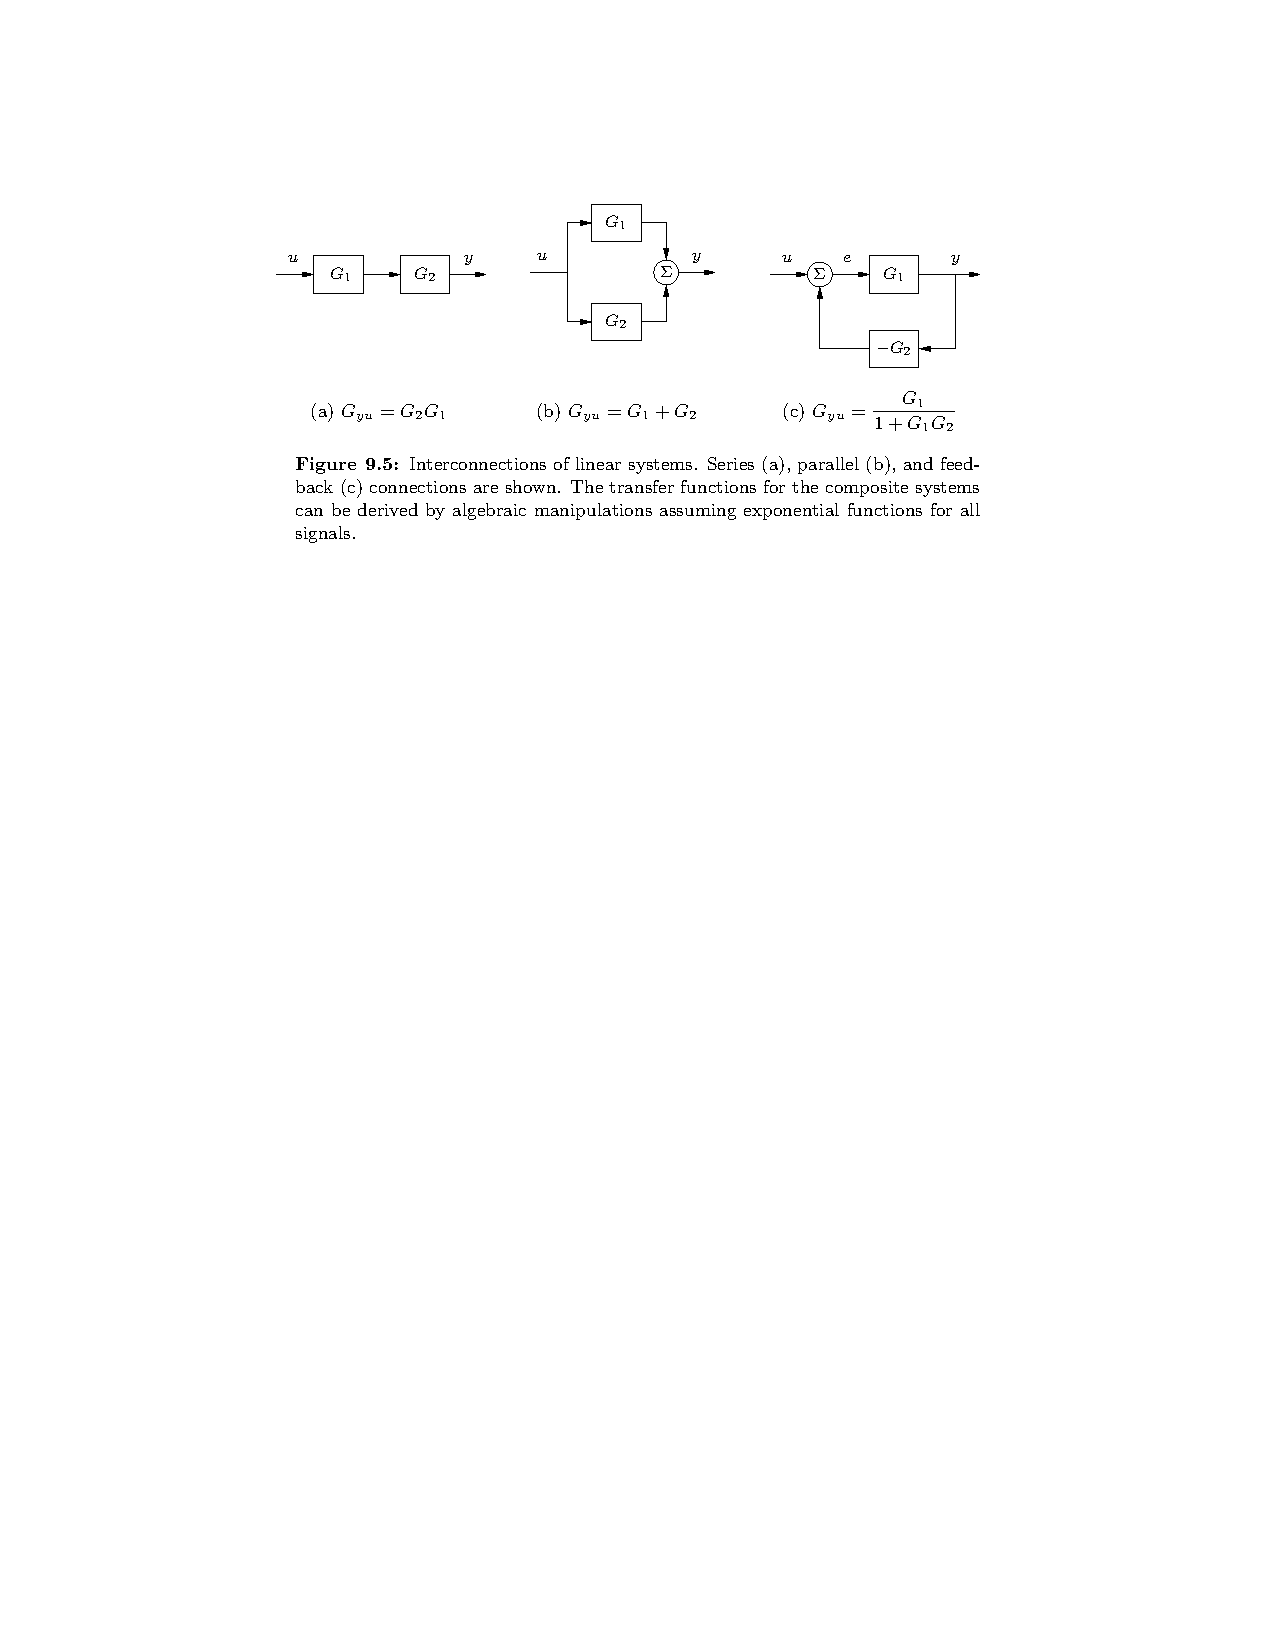
\includegraphics{figure9.5}

\end{frame}

\begin{frame}{Deriving the feedback loop}


\end{frame}

\begin{frame}{Block diagram algebra}


\end{frame}


\SUBCONCEPT{Control System Transfer Functions}

\begin{frame}{This is another slide}
\begin{itemize}
\item c
\item d
\end{itemize}
\end{frame}


\SUBCONCEPT{Algebraic Loops}

\begin{frame}{This is another slide}
\begin{itemize}
\item c
\item d
\end{itemize}
\end{frame}


\SUMMARYFRAME
\FINALE

\end{document}
